\chapter{Experimental Assessment of IaaS Clouds}\label{cap:evaliaas}
\noindent In this chapter we will be reviewing the most used frameworks to drive IaaS Clouds. An initial selection will be made and it will be progressively shrunk following certain criteria like maturity, ease of use or documentation quality, until only one remained. A deep study will be carried out on the prevailing last.

\section{Assessment Methodology}\label{sec:evaluacion}
\noindent A thorough evaluation of the capabilities of the different frameworks is not possible unless an actual deployment is carried through. The virtual infrastructure that is generated when a cloud has finished installing, no matter how small the deployment be, is large and complex. Besides, \emph{emulating} the hardware that will support the cloud is meager most of the times. \emph{Nested Hardware Virtualization} --- the capacity for a CPU to export its native virtualization capabilities to a guest running atop a host node, or the ability to use full hardware virtualization \emph{inside} a virtual machine ---, does not currently enjoy widespread adoption as it requires implementation efforts from both CPU designers and virtualization software developers. This means that it will not be possible for us to fully appraise the myriad IaaS Cloud solutions by creating a virtual cluster over which to deploy our clouds, and make performance measures.

To diagnose the superiority of one of them over the rest, a scaled down setup will be completed to evaluate the proficiency in maintaining the IaaS service running in spite of the reduced infrastructure. Quality and transparency in the documentation, as well as community support and engagement will also be borne in mind.

The testing environment follows the organization shown in figure \ref{fig:espacioprueba}.

\begin{figure}[tbp]
\begin{center}
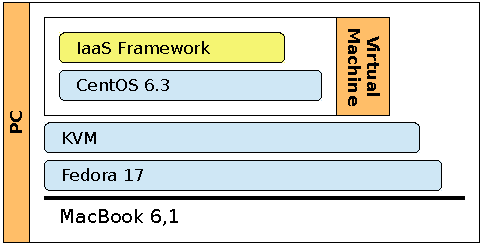
\includegraphics[width=0.55\textwidth]{imagenes/007.pdf}
 \caption{General testing environment}
\label{fig:espacioprueba}
\end{center}
\end{figure}

\section{Evaluated Frameworks}\label{sec:frameworksevaluados}
\noindent The frameworks are:
\begin{itemize}
 \item CloudStack %3.0.2
 \item Eucalyptus %3.1.1
 \item OpenNebula %3.8.1
 \item OpenStack
\end{itemize}

From an exclusively functional vantage point, the four of them clearly cover the requirements to run and manage the life cycle of an indeterminate number of custom VMs, through an API that would allow for the definition of a job control interface.

\emph{Eucalyptus} and \emph{OpenStack} take a more modular approach to the solution, unveiling smaller functional parts grouped in modules, while at the same time decoupling those modules from each other. With a module set in this fashion, installations become more flexible and tougher on par. However, to contain the operative effort, OpenStack ships with a series of scripts that help managing its deployments. Regarding their system requirements, they all support installations in modern Linux distributions with KVM or Xen as hypervisors. When dealing with a real deployment, which framework will be chosen will likely depend more on the existing platform than on particular limitations that any cloud may have.

As a side note, it is remarkable the lack of interoperability among them. All of them try to adhere to the AWS API in a different degree --- some of them support it partially, others use \emph{adaptors} to bridge their implementation to an AWS-compatible API. OpenNebula, OpenStack and Eucalyptus have demonstrated to be carrying on coding efforts to fully support the OGF's standard: OCCI.

%\subsection{Eucalyptus}\label{subsec:eucaliptus}

Eucalyptus, in spite of being the first to fully cover the AWS API, which is merely anecdotical nowadays, has two obstacles that hinder its evaluation. First, it is not fully open-sourced: \texttt{VMware Broker} which brings the opportunity to use virtualized infrastructure based on  VMware technology, is only available to paid subscribers. And second, it is impossible to setup Eucalyptus within a VM to test start-up time or installation complexity, for example, as it explains its installation guide \cite{eucainstall}. Both limitations make Eucalyptus back out from the evaluation list. The rest have been compared after their installation and configuration.

\subsection{CloudStack}\label{subsec:cloudstack}

\noindent CloudStack installation guide \cite{cloudstackquickinstall} describes the series of steps that a systems engineer should follow in order to complete a minimum CloudStack deployment. It clearly determines that Cloud Nodes' CPUs have to support virtualization extensions for CloudStack to start Xen or KVM-based VMs, which happens to be a similar limitation to Eucalyptus'. However, the fact that CloudStack would become part of \emph{The Apache Software Foundation} from version 4 onward \cite{cloudstackstrategy}, and the reality of a Citrix technical article opening the door to CloudStack deployments over Cloud Nodes lacking virtualization extensions \cite{apachecloudstack4}, made us arrange the layout shown in figure \ref{fig:cloudstack} to test-drive the CloudStack cloud implementation.

\begin{figure}[tbp]
\begin{center}
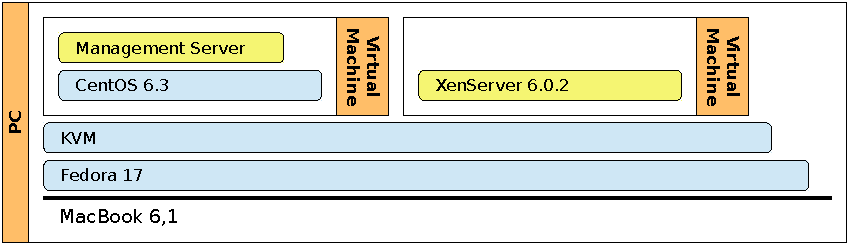
\includegraphics[width=0.99\textwidth]{imagenes/008.pdf}
 \caption{CloudStack 3.0.2 with XenServer hypervisor}
\label{fig:cloudstack}
\end{center}
\end{figure}

Following the advanced and quick installation guides --- \cite{cloudstackquickinstall} and \cite{cloudstackadvinstall} --- the process may be summarized in the steps below:

\begin{itemize}
 \item Two VMs were created to contain the CloudStack \emph{Management Server} (\emph{MS}) and the XenServer hypervisor: 1 GB of RAM for the MS, 3 GB of RAM for Xen, 20 GB HDD, \emph{ACPI} and \emph{APIC} for both.
 \item For the MS:
  \begin{itemize}
   \item \emph{CentOS 6.3} was downloaded, installed and \texttt{yum-updated}.
   \item The VM was named \emph{cloudstack}.
   \item Likewise, a user named \emph{cloudstack} was registered and added to the \emph{sudoers} list.
   \item The quick installation guide was followed to conclude the process.
  \end{itemize}
 \item For Xen:
  \begin{itemize}
   \item XenServer 6.0.2 was downloaded from Citrix web site.
   \item The notes section in the quick installation guide and in the XenServer configuration manual \cite{xenserverinstall} were followed to perform the configuration.
  \end{itemize}
  \item Additionally:
   \begin{itemize}
    \item Before specifying the execution environment a global flag had to be set to permit nodes with no virtualization extensions \cite{cloudstacknohvm} be part of the Cloud Nodes set.
    \item Once the configured infrastructure was online:
     \begin{itemize}
      \item The CentOS 6.3 image was uploaded to the MS.
      \item A \texttt{SimpleHTTPServer} --- a Python micro HTTP server --- was started on port \emph{443} in the MS.
      \item A rule was added in \texttt{iptables} to let traffic through on port \emph{443} in the MS.
      \item The VM image was loaded to the cloud from CloudStack's web interface.
     \end{itemize}
   \end{itemize}
\end{itemize}

\subsection{OpenNebula}\label{subsec:opennebula}

\noindent If balanced against the installation procedure just described, the effort for setting up OpenNebula 3.8 is lighter. The process that has been followed to configure the OpenNebula deployment contained in figure \ref{fig:opennebula} stems directly from \cite{centosonquickstart}, the official installation guide. The subsequent steps serve as summary to the process.

\begin{figure}[tbp]
\begin{center}
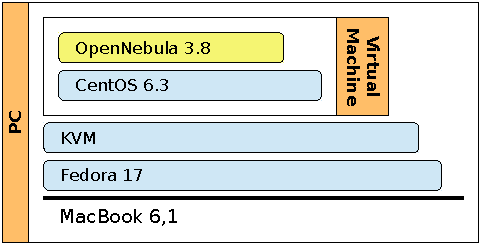
\includegraphics[width=0.55\textwidth]{imagenes/009.pdf}
 \caption{OpenNebula 3.8 with KVM}
\label{fig:opennebula}
\end{center}
\end{figure}

\begin{itemize}
 \item A supporting VM was created to fully contain OpenNebula: 1 GB of RAM, 8 GB for the HDD, ACPI and APIC.
 \item CentOS 6.3 was downloaded, installed and yum-updated.
 \item The VM was named \emph{opennebula}.
 \item A user named \emph{opennebula} was also registered and added to the sudoers list.
 \item \texttt{SELinux} was stopped.
 \item The configuration guide \cite{centosonquickstart} was followed to complete the process. Afterwards, the next series of actions were carried out to be able to test the framework:
  \begin{itemize}
   \item By default, OpenNebula's web interface module (\texttt{sunstone}) attaches to \emph{lo}. In order to interact with sunstone from outside of the containing VM, it was necessary to change the configuration file (\texttt{/etc/one}) so that sunstone attached to the external network interface \emph{eth0}. The very same happened with \texttt{occi}, the REST service that exposes the cloud API.
   \item Furthermore, iptables was modified for letting traffic through on port \emph{9869}; where sunstone listens by default.
  \end{itemize}
\end{itemize}

\subsection{OpenStack}\label{subsec:openstack}

\noindent OpenStack case is striking for many reasons. It represents the convergence of two different needs: the computationally-driven in NASA and the storage-bound in Rackspace. Complementarily, both Red Hat and Canonical had shown their interest in the platform by collaborating with their scripts, deploying utilities and cloud-optimized images.

Just as with OpenNebula, the complete execution environment was installed into a single VM. In this case, Fedora was chosen over CentOS or Ubuntu for the existence of a community-written installation guide \cite{quickstartfedoraos} and scripting utilities to ease the process.

Both Essex and Folsom versions were tested. The reasoning behind this is that in spite of being Essex the officially supported version in Fedora 17, the quick installation guide suggested using the latest version available --- Folsom by December 2012 --- enabling a testing repository to that end. The degree in maturity observed moving from Folsom to Essex was startling: not only the web interface had been revamped giving it a more thorough look that also reflected much better the state of the underlying infrastructure, under the hood, the core module had also been split in smaller functional pieces that could be easily distributed across the cluster. In Essex, when dealing with creating instances in the cloud, if there were any problem while the networking interfaces were being brought up, making it impossible for them to obtain IP addresses, the web interface would hang in a state that would not allow destroying the instance, requiring the invocation of console commands to fix the issue. This problem, for instance, is solved in Folsom.

An execution environment for both versions was spawned by following the next list of actions (see figure \ref{fig:openstack}):

\begin{figure}[tbp]
\begin{center}
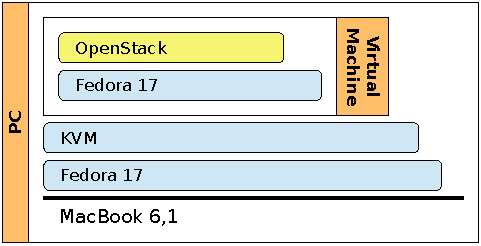
\includegraphics[width=0.55\textwidth]{imagenes/010.pdf}
 \caption{Virtual OpenStack deployment}
\label{fig:openstack}
\end{center}
\end{figure}

\begin{itemize}
 \item A single VM was created to hold OpenStack: 1 GB of RAM, 10 GB for the HDD, APIC and ACPI.
 \item Fedora 17 was downloaded, installed and yum-updated as usual.
 \item The VM was named \emph{openstack}.
 \item The \emph{openstack} user was registered as well as added to the sudoers list.
 \item \texttt{acpid} package was installed.
 \item SELinux was stopped.
 \item A full clone of the VM --- which includes the virtual drive --- was made to test both versions.
 \item The quick installation guide as well as the official one, omitting Swift, were followed to complete the process.
\end{itemize}

\section{Veredict}\label{sec:conclusiones}

\noindent What follows is the listing with the findings in comparing the frameworks according to the methodology described at the beginning of this section.
 
\begin{description}
 \item[Installation:] Without a doubt OpenNebula stands out in this regard. The installation guide is the lightest and shortest to follow with a difference. It carries, however, the inherent problem of hiding what is going on when it is being configured for the first time, potentially hardening the resolution of issues that might appear in the future.
 \item[Configuration and Management:] Growing the supporting cluster requires, on every cloud tested, that a compatible hypervisor be installed on any node added. CloudStack and OpenNebula offer a more transparent management interface to better control the physical infrastructure. OpenStack displays the most limited web interface.
 \item[Hypervisor:] Regarding hypervisor support, OpenStack clearly surpasses both CloudStack and OpenNebula. Yet, they all support the most widely used hypervisors --- KVM, Xen, Xen variants and VMware and variants --- in production deployments.
 \item[Storage:] The three of them support a broad assortment of data back-end controllers. But, in this case, it is important to highlight the effort OpenStack is involved in to introduce Amazon S3 compatibility in its deployments. Swift is the OpenStack component granting fault tolerance and high availability storage, mimicking Amazon S3, relying on data replication and balancing among other techniques. CloudStack advanced installation guide \cite{cloudstackadvinstall} describes a first approach toward configuring Swift as secondary storage for the cloud. This fact speaks volumes about the maturity and importance of Swift.
 \item[Documentation:] None of the three can boast about exhaustive official installation guides. Every framework has had its own exposure to different Linux distributions, so the coverage they offer varies to the point of mistaking module names; e.g., both CloudStack manuals are more easily followed using CentOS as base operating system and XenServer as hypervisor. OpenStack provides installation manuals supporting both Red Hat and Debian derivatives, but for Fedora the name of the services in the documentation does not correspond to the real ones; no such thing happened for Ubuntu. Nonetheless, inaccuracies are trivial to cope with and the manuals are deep enough to be used to make successfully deployments in production environments.
 \item[Community:] Even though it may seem unimportant, the community is vital for developing and supporting the frameworks. They are, at the very least, partially open-sourced, so a lively community translates into higher usage rates, more rigorous documentation, more bugs squashed, etc. While it is hard to assess the magnitude of an online community from the outside, it is interesting to highlight the nourishing that OpenStack is continuously receiving from Red Hat and Canonical: there is no technical keynote or conference in which OpenStack is not appointed.
\end{description} 

\subsection{OpenStack Folsom}\label{subsec:openstackfolsom}
\noindent The IaaS Cloud that has been chosen is OpenStack Folsom. The lengthy installation guides, the community support, the backing by two large software companies, the real deployments in production (from HP, Dell, Intel, Rackspace, etc.), the modular configuration, the completeness of the implementation (OCCI APIs, S3, EC2, Swift, etc.) and the \emph{official} support to deploying clouds over virtual clusters for testing have unbalanced the comparison in its favor.
